% \section{multi-tier Fog computing model}
% \label{sec:fog-model}

\subsection*{Research Goals}
\label{sec:research-goals}

Considering a reliable and high-quality video delivery architecture to be used in the Smart City environments~\cite{gamaUCC2019}. The proposed scheme will take advantage of several network-related technologies such as Cloud, Fog, and Edge Computing, as well as intelligent microservice placement and chaining. Figure~\ref{fig:scenario-arch}~(left-side) depicts a multi-tier network architecture, which is composed of a heterogeneous set of devices and applications using the resources and also offers a multi-access communication technology, such as 5G and WiFi. Based on these premises, as a novelty, we consider users to have a simultaneous multipath connectivity in different nodes~\cite{poliakovPHD2018}.
On the right-side we describe a part of the parameters that should be assessed to define what microservices need to be deployed and what is the most suitable tier to deploy them. Notice that the parameters is down tier for feedback is distinct of the others tiers.
The assessed parameters include, but are not limited to, the user's profile, the load of the local cell, the link quality, the motion complexity of the videos, and also smart city details such as the location and the traced route in case of users with mobility. Some of the nodes can be stationary, but others can range from low to high mobility patterns. %In order to take into consideration all these details, the proposed methods will have to fetch information from the routing protocols as well as the cell and subscriber radio interface information, such as location, cell load, and link quality.
%, the type of the video application (eHealth, entertainment, augmented or virtual reality, 360 videos), the motion complexity of the videos, and also smart city details such as the location and the traced route in case of users with mobility. To take into consideration the node’s mobility. Some of them can be stationary, but others can range from low to high mobility patterns. In order to take into consideration all these details, the proposed methods will have to fetch information from the routing protocols as well as the cell and subscriber radio interface information, such as location, cell load, and link quality.

\vspace{1cm}
\begin{figure*}[htpb]
	\centering
	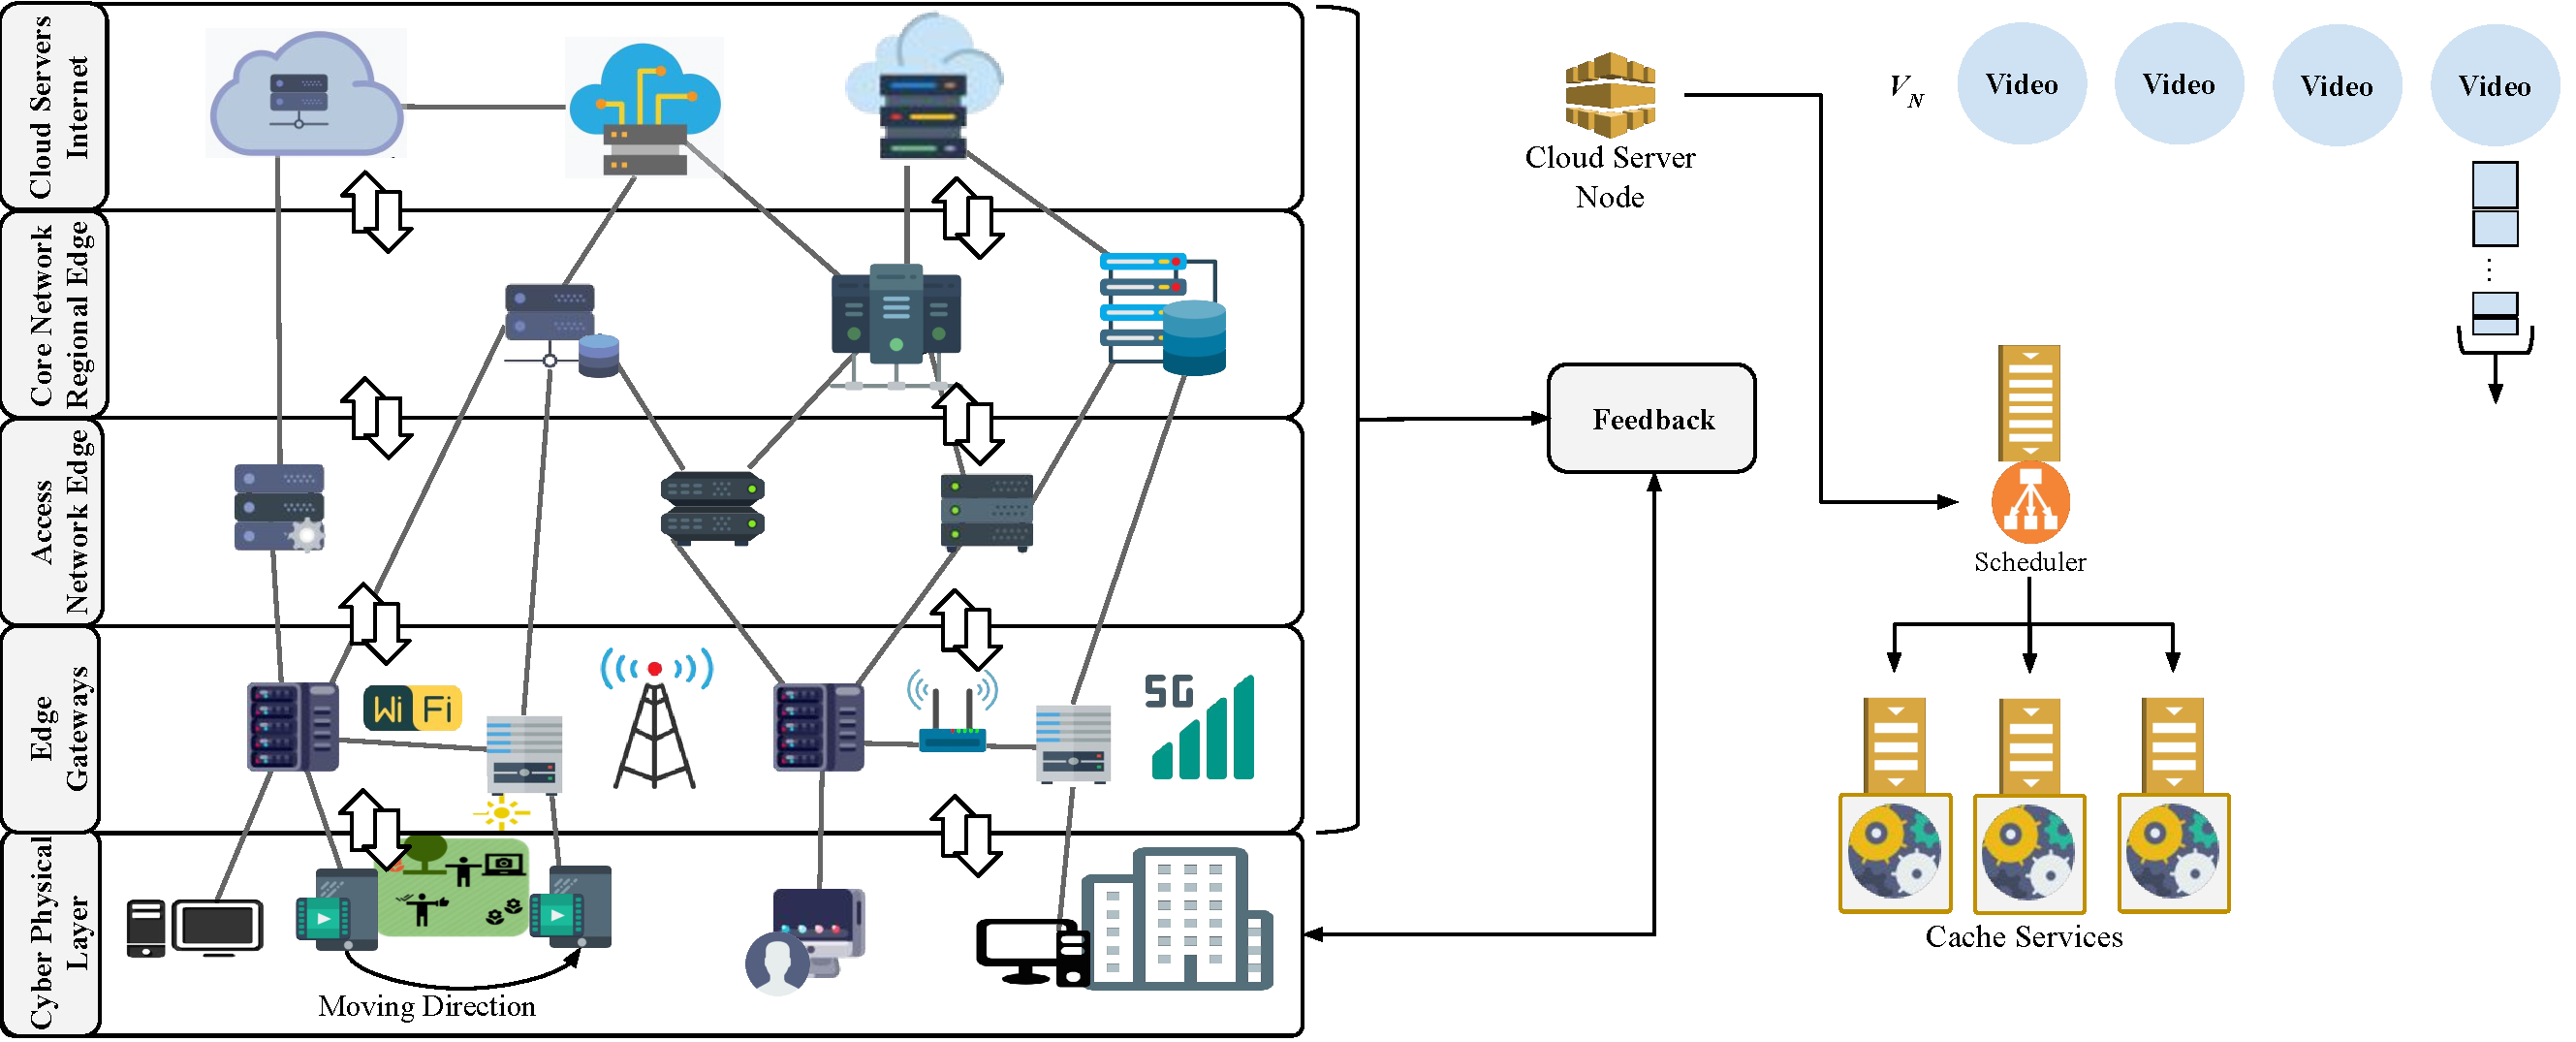
\includegraphics[width=1.0\textwidth]{images/scenario_incomplete}
	\vspace{-1cm}

	\caption{DASH-based Adaptive Multimedia Delivery System in an Smart City Envirnment.}

	\label{fig:scenario-arch}
\end{figure*}
% The experiments will be implemented using the simulation software ns-3 (http://www.nsnam.org) to create a multi-tier Edge/Cloud Computing environment. existing ns-3 models are quite diverse and have a rather loose compatibility between each other. The ns-3 community provides MPEG-DASH implementations and support mobility.%, it happens that they are not directly usable due to incompatibilities. In this work, we present an ns-3 distribution that packages the AMuSt Framework DASH implementation [81]

% The first tool that will be used is Docker. It allows to create, configure, and run containers, which is a lightweight way to provide isolation, automation, compatibility, and integration of services. The second tool is Kubernetes. This is a container-orchestration platform to automate several container-related activities, such as automatic deployment, management, scaling, and operations between different clusters and hosts. JUJU is a modeling tool to perform quick deploys of container-based applications in several private and public cloud services. It also helps to configure, interact, and easily perform several other operational tasks. In addition, the 5G-EmPOWER will be used to provide Multi-access Edge Computing support with heterogeneous radio access technologies and lightweight virtualization.

%Description of the work you'd like to do, as well as the expected outcomes and results.

Given the aforementioned multi-tier edge/cloud environment and service architecture, this work aims to tackle the following research questions expected:
\textit{i)} Build an hierarchical adaptive multimedia delivery system to analyze the influence of chunk size variation on bitrate adaptation hierarchical scheduling algorithm; \textit{ii)} How to determine the best tiers to place microservices; \textit{iii)} Facilitates video streaming through multiple sources; 
\textit{iv)} Use location information to estimate best paths/gain/ in real time of edge servers. How to dynamically estimate the gain between the different close perspective of the proximity of the servers. You need to redistribute unsolicited content or just add content on other edge servers when user changes server? Which one should we do this?
%A video system becomes more robust since multiple points of failure are inserted, enhancing availability; ii) increase in reliability since the information that passes through the network is not stored by the intermediate node; iii) Facilitates video streaming through multiple sources; 


%Neste trabalho, queremos construir mecanismo para um sistema de distribuição adaptativo multimidia baseado em DASH, buscando o otimizar sua topologia de forma adaptativa para minimizar a latência de reprodução média e melhorar a entrega do fluxo de forma oportuna. 
%Neste trabalho, queremos construir um sistema CDN na fog com o uso de cache e sobreposição
%de rede para para streaming de video ao vivo, e otimizar sua topologia de forma adaptativa para
%minimizar a latência de reprodução média e melhorar a entrega do fluxo de forma oportuna.
%A latência de reprodução é a diferença entre o tempo de reprodução (ponto de reprodução) na
%origem de midia e em um nó.
%Modelagem de propriedades de balanceamento de carga e desempenho de cache
%em sistemas de Névoa-Nuvem multicamadas.
%1. Interesses perspectivas do usuário, provedor de serviços e provedor de rede.
%2. Qual a melhor forma de operar problemas de cache em névoa-nuvem? Onde? Quando?
%Como?
%3. Redimensionar recursos necessários para suportar demanda de Acordo com o tempo.
%4. Utilizar máquinas virtuais (container, microservices) para atingir a latência minima para
%acelerar a execução do escalonamento, mas irá implicar em desperdicios de recurso (e
%dinheiro)? Caso sim, como minimizar este desperdicio?
%
%Suporte a mobilidade.
%1. Quais mecanismos devemos utilizar/desenvolver para lidar com a mobilidade do usuário?
%Como dividir o conteúdo e recursos computacionais?
%2. Como utilizar a informação de localização para estimar melhores caminhos/ganho/ em
%tempo real dos servidores de borda. Como estimar dinamicamente o ganho entre as dife-
%rentes perspectivas da proximidade dos servidores.
%3. É necessário re-distribuir o conteúdo não requisitado ou apenas adicionar o conteúdo em
%outros servidores de borda quando o usuário muda servidor? Quais nós devem fazer isso?
%4. É necessário possuir nós reservados extras e prontamente disponiveis com intuito de re-
%dundância de recurso computacional?
%5. Antes de escolher um provedor de IaaS para alocar máquinas, quais serviços é necessário
%acrescentar para o provisionamento do conteúdo?

%\begin{enumerate}
%	\item We aim to build an hierarchical adaptive multimedia delivery system to analyze the influence of chunk size variation on bitrate adaptation scheduling algorithm performance.
%\end{enumerate}
%In this proposal, we aim to build an hierarchical adaptive multimedia delivery system to analyze the influence of chunk size variation on bitrate adaptation scheduling algorithm performance. Based on the features of HTTP-based adaptive video streaming, we build a general model for debloy a cooperative video streaming delivery, which may be used in D2D in mobile network, regional networks using Points of Presence as nodes, during flash crowds where having upload bandwidth alone is not sufficient to accommodate the flash crowd as the nodes take time to locate the available resources.


% The other three levels represent the network mist / edge. This work takes into account edge nodes with computational capacity and storage, and classifies them hierarchically according to their coverage and communication technology [?]. In a multi-level ecosystem, the Core Network Regional Edge can perform management within a city, for example, baseband unit (BBU) and Internet service provider (ISP). The Access Edge Network, which supports a few dozen or perhaps a few hundred local nodes in the fog, can be represented by a Base Station or Access Point. Edge Gateways can be deployed on local fog nodes such as personal computers, laptops, and smartphones where the node delegates video content over wi\reless connections.

% Research goals, including a problem statement.
%Currently the Internet is based on the characteristics of the best effort (Best-Effort), with no guarantee of level of service, beyond that, the congestion control and the lossless through rate-based transfer for conflict-free matching is deployed in IP layer. The existing schemes suitable for chunk delivery cannot be directly utilized in PoPs due to several issues:
%\textit{i)} One chunk may have several copies, which impacts on the selection of origin servers; \textit{ii)} Defferent chunks can have distinct impacts on thre Quality of Experience~(QoE), e.g., initial delay and smoothness, which is crucial to chunk transfer but not considered in the original schemes~\cite{shenIWQoS19}.



%The main goal of this project is to design, implement, and assess a reliable and high-quality multi-tier video delivery architecture to be used in the Smart City environments. The proposed scheme will take advantage of several network-related technologies such as Cloud, Fog, and Edge Computing, as well as intelligent microservice placement and chaining. Figure 1 depicts a multi-tier network architecture, which is composed of a heterogeneous set of devices and applications using the resources and also offers a multi-access communication technology, such as 5G and WiFi. Based on these premises, a multitude of parameters should be assessed to define what microservices need to be deployed and what is the most suitable tier to deploy them. In addition, network slices also should be defined, created, configured, or re-arranged based on these parameters. The assessed parameters include, but are not limited to, the user’s profile, the load of the local cell, the link quality, the type of the video application (eHealth, entertainment, augmented or virtual reality, 360 videos), the motion complexity of the videos,
%
%
%We are going to deploy some experiments in The Stable Marriage Problem in the parallel Multipoint-to-Multipoint (MP2MP) transfer scenario in order to improve the QoE in DASH chunk delivery in hybrid scenarious. 
%Considering that each particular scenario has its own requirements, there is no one-to-one relationship between all classes of applications presented here and all classes of constrained devices presented in Section 2.1.
%
%The proposed model enables the provision of dynamically deployed sets of multimedia services in fog/cloud environments. Users can access such services by various communication technologies (e.g., 4G, 5G, WiFi, etc.). In scenarios like this - which normally make up the network haze - they may have edge nodes that also provide computing and storage services [?], [?]. For this, we first introduced a multi-tier architecture, detailed in Figure 1. The highest tier is comprised of cloud servers, which may be located in public or private clouds. Clouds may be, for example, an on-demand video provider.


%
% ===========================================================================================
%
% Having upload bandwidth alone is not sufficient to accommodate the flash crowd as the nodes take time to locate the available resources. The framework solution can be used to assist the content providers joinging the content in the edge of the network, in this way, the regionals networks may attend the end-users. Moreover, due to intense competition among the nodes, this available bandwidth is also not fully utilized. Based on these, various population control measures have been suggested for both mesh-based and tree-based systems.

% Content delivery in wireless caching networks via device-to-device (D2D) communications can effectively offload the traffic burden and reduce the delivery delay and the energy consumption

%\subsection{Network Model}
%
%Currently the Internet is based on the characteristics of the best effort (Best Effort), that is, there is no guarantee of level of service. However, users often need to use the services made available in the cloud with a QoS guarantee, which is specified in a contract known as a Service Level Agreement (SLA). In other words, SLA is a document agreed between two or more entities in which the description, delivery and collection of contracted services are formally defined.
%
%In addition, there are many pragmatic trade-offs in edge provisioning. In addition to meeting the purpose of proximity between users and edge servers, edge operators also consider cost budgets, the ability of edge sites, provisioning edge site interrupts, and constraints that users can work on. regional laws or policies of ISPs. These considerations usually fit well together, resulting in a huge research space. Edge operators should consider these offsets comprehensively and exploit the best provisioning plan under various constraints
%
%In addition, a common problem with the video stream provisioning mechanism in CDNs, where CDN nodes in fog should be encouraged to share their resources and contribute to the content design. This can have a serious impact on the quality of streaming system service. Existing solutions address the problem by categorizing following way:
%
%\begin{itemize}
%
%	\item \textit{Monetary base}
%	\item \textit{Based on reciprocity}
%	\item \textit{Based on Reputation}
%	
%\end{itemize}
%
%% ========== OLD TEXT =====================
% A uso da computação em névoa para a distribuição de conteudo CDN pode ser vital para a good QoS and QoE garantees. In these kinds of scenarios - that make up the fog network - may be any access points (AP) can be extended to also provide computing and storage services. The APs may be any device that offers wired/wireless network connection to the end-user, such as smart phones, tablets, laptops, connected vehicles.% Cite bit paper 
%
%To clarify the possibilities, we first introduce a multi-tier fog computing model detailedly in Figure \ref{fig:fog-model}. As we can see, the higher tier is composed by the Provider that offers video streaming services (e.g. Netflix, Amazon, Youtube) located at the cloud, and makes either use of their own cache systems or leases one offered by CDN providers. %(... CDN providers: Akamai, CloudFlare, Rackspace, Amazon's AWS, MaxCDN CDN nodes)
%These providers operate original content in datacenters at the WAN (long-haul netwoks). In fog network, the APs located at the fog are responsible to provisioning resources to CDN providers allocate their caches. Notice that the caches are to multi-hop away from the content provider/consumer. A very popular fashion to organize the cache placement content hierarchicaly, and bi-directional communication. In addition, each content pode ser splitted dynamically in a set of pieces in order to serve the end-users, taking into account different aspects, such as the mobility presented by the user and the possibility to predict the moving directing. 
%
%With new possibilities being created to offer better services and the working of the internet. As long as the network becomes more robustness, the problem become more complex and new challenges arises to be solved. To tailored a CDN systems with multi-tiers environment into the fog, different characteristics have to be studied such as cache allocation, placement, replacement and selection caches, usually, making real-time decisions. As different cache sizes being allocation over the tiers to storage a range of content to provisioning a region. Also, an cache size in an AP device have to be able of deal a set of different content pieces, in order to the end-users may have QoE garaties. Thus, different level of granularity into the APs devices arises, if the granularity of certain areas becomes too fine, scalability issues begin to appear. Dividing the content of the fog in the network over the APs at the right level of granularity is a complex problem in its own right.
%% map unit (Algorithmic Nuggets in Content Delivery)
% 
%% An network can be represented by a $(n+2)$-partite graph with $G = N_{c} \cup ( \bigcup_{i}^{N} V_{f}^{i}) \cup V_{d}$ 
%
%For retrieve a data afetwards a VM (or content, service, etc) being allocated or allready exists. The operations feitas pela aplicação podem ser receiver-driven, such as used in Content-Centric Network (CCN) and named data network (NDN) paradgm. 
%Organizadas de hierarquiquamente, one content object name could be retrive trough an url name "ucla/videos/demo.png". For a large video that is shareded em a set o chunks, thereby  que uma requisiçao pode ser feita especificando um chunk do video  da seguinte foma "ucla/videos/demo.png/1".
%
%Um provedor de conteudo possui a set of repositorios CDN geograficamente distribuidos. As requisições dos usuarios para conteudos geralmente são feitas atraves de HTTP GET requests. To provisioning the content, the CDN redirects the request through either DNS redirection [38] or IP-layer anycast [41]. 
%
%O conteudo provido por repositorios CDN geograficamente distribuidos, visando estar proximo ao usuario. Procura melhorar o troughput da rede. Mas para isso o provedor do conteudo alvo.  CDN system
%
%%\begin{figure}
%%	\centering	
%%    \includegraphics[width=\linewidth]{images/router-processing-flow.pdf}
%%	\caption{State machine of rountig operation.}
%%    \label{fig:fog-model}
%%\end{figure}
%    
%\section{Business model perspective}
%
%A flexibilidade ao utilizar da edge networks infrastructure oferecem new oportunidades para melhorar o servico, abordando metricas e perspectivas que geralmente são analisadas de forma independente. It can be seen in three different perspectives:
%
%% Look at Offloading Content with Self-Organizing Mobile Fogs reference, present three respectives business ains and costs.
%
%\begin{itemize}
%
%\item \textbf{End-user perspective:} uninterrupted connectivity and communication services, smoth consumer experience.
%
%\item \textbf{Content provider perspective:} connected intelligent 	transportation systems, road-side service units, sensors, and mission critical monitoring/traking services.
%
%\item \textbf{Network operator perspective:}  scalable, energy- efficient, low-cost, uniformly-monitored, programmable, and secure communication infrastructure.
%
%\end{itemize}
%
%\section{Distribution of Information Centric}
%
%
%\section{CDN Slicing Architecture}
%\label{sec:cdn-slicing-archi}
%
%This CDN service based on fog computing consider the scenarios presented in Fig. \ref{fig:fog-model}. This section is interested in make up an architecture capable to provisioning this service in on-demand manner. In order to investigated aspects as scalability over the live migration, granularity of different contents and providers, aside from mobile predictability considering the social medias and moving direction. Initially, the model at the Fig \ref{fig:intro} shows two layer components: the user device, fog nodes into the multi-tier APs and the cloud providers. 
%
%The usage of CDN multi-tier fog platform rather than the cloud CDN have to be consider, mainly, the cost reduction.
%The Edge server placement problem is responsavel de selecionar um nó na borda da rede. 
%There will exists two kind of nodes in the network, which are both known and unknown nodes due to the flexibility presented by the edge. The edge node location could respresented by a tuple da $<< city, AS(Autonomous\ System)>>$. let us assume that in current scenario a set of files $S = \{s_{1}, s_{2}, ..., s_{n}\}$ 
%
%The problem to cost minimization could be reducted to the problem "the optimal bandwidth allocation problem" (OBAP), described in [].
%
%The cost of a solution could range of an agreement with a CSP. As the focus of CDN apps are high in/out of datas, this work leverage the concerns of price machines needed to the CDN utilization and the charge of fog  networks, aside from the cost of download and upload files in order to sync different nodes and distribute the files to end-users.
%
%For provide a high-quality experience sharing into the same regional APs, the model 
%
%For provide a high-quality experience general components have to take advantage of the moving direction presented by the user. This way, the monitoring and analytics modules may cooperate togheter with advanced machine learning, neural networks techniques for decision-making. Characteristics as users location, direction movement, users behaviour, content resquested, amount of stored data, data traffic needs, cloudlets capacity, newotrk capacity, and so on.
%
%make location-based virtual machine migration feasible in the Fog computing paradigm.
%
%to build pro a hierarchical, bi-directional computing infrastructure: edge devices communicate with cloudlets and cloudlets communicate with clouds. Cloudlets can also communicate with each other to perform data and process management in order to support application requirements, and to exchange Fog control/management data (such as user device and application state).
%
%
%%an architecture thet offer CDN as a Service (CDNaaS) on demand over the end-users have to take some decisions, such as resource allocation, placement, real-time management decisions, maintaining the service level agreement.
%
%
%al-time management decisions, maintaining the service level agreement.
%
%With the possibility to provision algorithms as a set of function trough VNFs to provision end-user  some service, CDNaaS may be decouple in specific functions which will be orchestrate over the network to provision QoE garantees for end-users. Below presents an Architecture standard ETSI for CDN.
%
%To deliver an efficient CDNaaS into an heterogeneos network environment with multi tier fog nodes, our envisioned architecture showed up in Fig 1 is composed by a cloud provider where is contented big datacenters, from here the when the user request a movie. The fog computing may be organized hierarquicaly by multiple levels from which serve como meio de prover o serviço de CDN. As can be seen in fig 1 an user 1 receiving a content from WiFi and the another user is receiving from both LTE and user 1.
%
%The most recently CDN architectures highlight Network Function Virtualization (NFV) principle para permitir a execução de serviços especificos em servidores remotos. Accorndlying to [], NFV supports a wide range of services by orchestrating the VNF (virtual network function) deployment and operation across diverse computing, caching, and networking resources over the multi-tier fog nodes. Whereas SDN  paradigm decouples the control plane from the underlying data plane in a centralized manner. It is independent from NFV, but it can add more flexibility to the SFs. Therefore, a  hybrid  concept  may  exploit  both  NFV  and  SDN  at  the same  time.  Virtualization  concepts  are  integrated  in  different areas such as cloud and telecommunication for more services flexibility provisioning. This combination technology may be deployed as virtual machines capable to provision slices of CDN components on-the-fly in a dynamic manner [2][3]. This way, whenever CDN as a Service (CDNaaS) may be offered on demand for the end-users. In addition, the use of NFV and SDN jointly can take advantage of an platform prepared to deal with an multi-tier edge environment. %SDN  paradigm  then  decouples  the  control  plane  from  the underlying data plane in a centralized manner. It is independent from NFV, but it can add more flexibility to the SFs. Therefore, a  hybrid  concept  may  exploit  both  NFV  and  SDN  at  the same  time.  Virtualization  concepts  are  integrated  in  different areas such as cloud and telecommunication for more services flexibility provisioning.
%%Logical partitions in NFV is also known as resource slicing, which divides the network into slices made of different resources and capacities so as to offer differen- tiated services for heterogeneous use cases and enable creation of customized services with fine control fea- tures of QoS [7, 8, 12, 13].
%
%%\begin{figure}[!t]
%%	\centering
%%    \includegraphics[width=\linewidth]{images/archi-ETSI.pdf}
%%	\caption{Experimental setup for the spatial-based methodology.}
%%    \label{fig:intro}
%%\end{figure}
%
%which delivery the distributed content,
%
%it is needed instantiate VNFs that may replace virtualization services among de nodes in defirent tiers of the network. This way 
%
%With the Needed of download high quality multimedia content by the mobility users, this section introduces an architecture multi-tier composed by heterogeneous wireless network access (fig). Due to propogation of a In a network The devices  Due to the diference of range among the devices such as Cloud, ISP, LTE, WiFi, D2D. 
%
%introduces an architecture composed of a cloud computing (Tier 1) together with multi-tier fog nodes (Tiers 2, 3, and 4), which work collaboratively to enable service migration for video distribution with QoE support. In such architecture, we consider fully connected and fully fog-enabled scenario, where fog nodes are hierarchically organized to provide video services for end-users. There may be widely distributed local fog nodes, e.g., mobile devices (i.e., Tier 4), where such fog node relays the video content via device-to-device (D2D) wireless communication for mobile devices with high and similar traffic demands could cooperate with each other to form a D2D network. The neighborhood fog node, e.g., Base Station (BS) or Access Point (AP) (i.e., Tier 3), supports a few dozen to perhaps a few hundred local fog nodes. Above these would be regional fog node, e.g., baseband unit (BBU) or Internet Service Provider (ISP) (i.e., Tier 2), managing city-wide coordination. On the top of such multi-tier architecture, there is the cloud (i.e., Tier 1). 
